\documentclass{standalone}

\usepackage{tikz}
\usetikzlibrary{calc}

\begin{document}

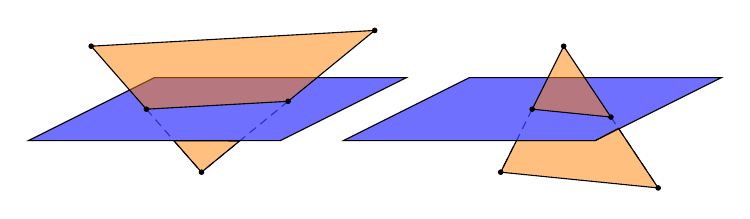
\begin{tikzpicture}[scale=0.8]

\begin{scope}
\coordinate (O)  at (0,0);
\coordinate (P1) at (-3,-0.5);
\coordinate (P2) at ($(P1)+(2,1)$);
\coordinate (P3) at ($(P2)+(4,0)$);
\coordinate (P4) at ($(P3)+(-2,-1)$);
\coordinate (Q1) at (-2,1);
\coordinate (Q2) at (2.5,1.25);
\coordinate (Q3) at (-0.25,-1);

\draw[densely dashed] ($0.5*(Q2)+0.5*(Q3)$)--(Q3);
\draw[densely dashed] ($0.5*(Q1)+0.5*(Q3)$)--(Q3);
\filldraw[black, fill=blue!75!white, fill opacity=0.75] (P1)--(P2)--(P3)--(P4)--cycle;
\filldraw[black, fill=orange, fill opacity=0.5] (Q1)--(Q2)--($0.5*(Q2)+0.5*(Q3)$)--($0.5*(Q1)+0.5*(Q3)$)--cycle;
\filldraw[black, fill=orange, fill opacity=0.5] (Q3)--($0.25*(Q1)+0.75*(Q3)$)--($0.22*(Q2)+0.78*(Q3)$)--cycle;

\foreach \pt in {Q1,Q2,Q3}{
	\draw[fill=black] (\pt) circle (1pt);
}
\draw[fill=black] ($0.5*(Q2)+0.5*(Q3)$) circle (1pt);
\draw[fill=black] ($0.5*(Q1)+0.5*(Q3)$) circle (1pt);
\end{scope}

\begin{scope}[xshift=5cm]
\coordinate (O)  at (0,0);
\coordinate (P1) at (-3,-0.5);
\coordinate (P2) at ($(P1)+(2,1)$);
\coordinate (P3) at ($(P2)+(4,0)$);
\coordinate (P4) at ($(P3)+(-2,-1)$);
\coordinate (Q1) at (0.5,1);
\coordinate (Q2) at (2,-1.25);
\coordinate (Q3) at (-0.5,-1);

\draw[densely dashed] ($0.5*(Q1)+0.5*(Q3)$)--(Q3);
\draw[densely dashed] ($0.5*(Q1)+0.5*(Q2)$)--(Q2);
\filldraw[black, fill=blue!75!white, fill opacity=0.75] (P1)--(P2)--(P3)--(P4)--cycle;
\filldraw[black, fill=orange, fill opacity=0.5] (Q3)--(Q2)--($0.42*(Q1)+0.58*(Q2)$)--(P4)--($0.25*(Q1)+0.75*(Q3)$)--cycle;
\filldraw[black, fill=orange, fill opacity=0.5] (Q1)--($0.5*(Q1)+0.5*(Q2)$)--($0.5*(Q1)+0.5*(Q3)$)--cycle;

\foreach \pt/\pos in {Q1/above,Q2/right,Q3/left}{
	\draw[fill=black] (\pt) circle (1pt);
}
\draw[fill=black] ($0.5*(Q1)+0.5*(Q3)$) circle (1pt);
\draw[fill=black] ($0.5*(Q1)+0.5*(Q2)$) circle (1pt);
\end{scope}

\end{tikzpicture}

\end{document}